\documentclass[10pt,a4paper]{article}
\usepackage[margin=1.55cm]{geometry}
\usepackage{helvet}\renewcommand{\familydefault}{\sfdefault}
\usepackage{graphicx,booktabs,xcolor,fancyhdr,float,array,enumitem}
\usepackage[hidelinks]{hyperref}
\definecolor{bigorange}{RGB}{255,130,0}
\definecolor{biggrey}{RGB}{60,60,60}
\pagestyle{fancy}\fancyhf{}
\lhead{\textbf{\color{bigorange}Banco BIG} \color{biggrey}| Rates Research}
\rhead{\color{biggrey}\today}
\cfoot{\color{biggrey}\thepage}
\renewcommand{\headrulewidth}{1pt}
\setlength{\parindent}{0pt}\setlength{\parskip}{4pt}
\newcommand{\sect}[1]{\section*{\color{bigorange}#1}}
\newcommand{\code}[1]{\texttt{\small #1}}
\begin{document}

\begin{center}
{\LARGE\textbf{\color{biggrey}Positioning Composite --- Normalization Versions}}\\[3pt]
{\color{bigorange}\rule{\textwidth}{2.5pt}}\\[3pt]
{\small Five interchangeable composite methodologies on one signal: the current triple-normalization
baseline, a single-standardization Kaiser-PCA, the CFTC/Street best-practice, a single-pass EWMA/52w, and
a two-dimension curve read. Built concurrently against one fixed data interface; the production default is
unchanged.}
\end{center}

\sect{1. Why and what}
The audit showed the live composite is $\sim$13 months slow because normalization is a triple pass
(rolling-3y-z of the level $\to$ \code{StandardScaler} $\to$ PCA $\to$ rolling-3y-z of PC1). This note
rebuilds the composite five ways --- each a self-contained module in \code{positioning/versions/} coded
against a fixed \code{base.py} interface (shared inputs: DV01-weighted per-category net positions, open
interest, curve books, yields; shared normalizers), so they are directly comparable and \emph{selectable}
via \code{get\_composite(version)}. \code{positioning/core} and the live \code{positioning\_score.json}
are untouched. Sign convention throughout: positive $=$ crowded net long duration (curve: $+ =$ steepener).

\sect{2. The five versions}
\textbf{V0 --- Production (baseline).} Rolling-3y-z features $\to$ PCA (fit 2006--19, 2 fixed PCs) $\to$
rolling-3y-z of PC1. Latest $z=+2.49$.

\textbf{V1 --- Kaiser-PCA (single standardization, eigenvalue$>$1).} \emph{The requested fix.} Raw
per-category net-DV01 levels, standardized \emph{once} (\code{StandardScaler} fit on the 2006--19 train
slice, projected forward), PCA on the same slice, retain PCs with \textbf{eigenvalue $>$ 1 (Kaiser)};
composite $=$ PC1 read straight off the projection --- \emph{no} rolling re-z. Result: eigenvalues
$[2.05,\,0.91,\,0.04]$, so \textbf{one PC survives} (PC1 $=$ 68.3\% of variance; PC2 at 0.91 just misses
Kaiser, so no separate curve factor here). Removing both rolling passes is exactly what kills the lag.
Latest $=+7.71$ --- legitimately large because PC1 is unit-variance on the \emph{pre-2020} window and
today's book is a multi-year extreme \emph{outside} that window; V1 does not re-normalize that away
(unlike V0). Read V1 as ``distance from the pre-2020 normal'', not as a rolling z. (A documented
\code{raw\_cov} sub-variant --- PCA on the unscaled covariance --- is dominated by the largest-variance
series, asset managers, confirming why standardizing first matters.)

\textbf{V2 --- CFTC / Street best-practice.} The industry method: on the DV01/10y-equivalent buy-side net
(the OFR convention), a bounded \textbf{COT-index} $=$ mean of the 52w and 3y min-max stochastics
($0$--$100$, crowd $>$80), with an unbounded \code{street\_z} $=0.5\,z_{52}+0.3\,z_{\%OI}+0.2\,z_{flow}$
in support (52w z; net-\%-of-open-interest z; 13w flow z). Latest COT-index $=\mathbf{85.5}$ (crowded);
sub-readings cot$_{52}=81.6$, cot$_{156}=89.4$, $z_{52}=1.39$, $z_{\%OI}=1.48$, $z_{flow}=-0.64$,
\code{street\_z}$=1.01$.

\textbf{V3 --- EWMA / 52w single-pass.} The simplest low-lag composite: $0.7\times$ EWMA-z (half-life
26w) $+\,0.3\times$ 13w-flow z of the buy-side level. One standardization, no PCA. Latest $=+0.61$
($z_{52}=1.39$, EWMA-z$=1.14$) --- already easing because flow turned negative.

\textbf{V4 --- Curve, two dimensions.} Splits the steepener/flattener read into \textbf{book tilt} (raw
front$-$long DV01, currently $\approx-2.6$ \$mm/bp $=$ flat) vs \textbf{momentum} (EWMA-z, $+1.42$
steepener-direction); plus a PCA slope factor ($-1.40$; its eigenvalue $0.22<1$, so it is a diagnostic,
not Kaiser-retained) and a COT-index of the curve book ($95.2$, near its 52w top). Resolves the earlier
``$+1.46$ crowded steepener'' ambiguity: the \emph{book} is flat; only the \emph{momentum} is steepening.

\sect{3. Responsiveness --- the whole point}
Same underlying signal, when did each first flag ``crowded'' in the current build-up:
\begin{center}\begin{tabular}{llccc}
\toprule
Version & Metric & Latest & First ``crowded'' flag & Lead vs production\\
\midrule
V0 Production & 3y double-z & $+2.49$ & 2026-01-20 & ---\\
V1 Kaiser-PCA & single-std PC1 & $+7.71$ & 2024-06-04 & \textbf{$+$85 wks ($\sim$20m)}\\
V3 EWMA/52w & EWMA-z $+$ flow & $+0.61$ & 2024-08-13 & \textbf{$+$75 wks ($\sim$17m)}\\
V2 CFTC/Street & COT-index (0--100) & $85.5$ & 2024-12-24 & \textbf{$+$56 wks ($\sim$13m)}\\
V4 Curve & momentum (curve, not duration) & $+1.42$ & 2026-03-03 & n/a (different signal)\\
\bottomrule
\end{tabular}\end{center}
Every duration-crowding alternative flagged the crowd \textbf{13--20 months} before the production
composite. The tell: V1/V3 have already \emph{peaked and are rolling off} while V0 is only now printing
its high --- the 3y double-z is a rear-view mirror. (V4 is the curve dimension; its ``lead'' vs a
duration metric is not comparable.)

\begin{figure}[H]\centering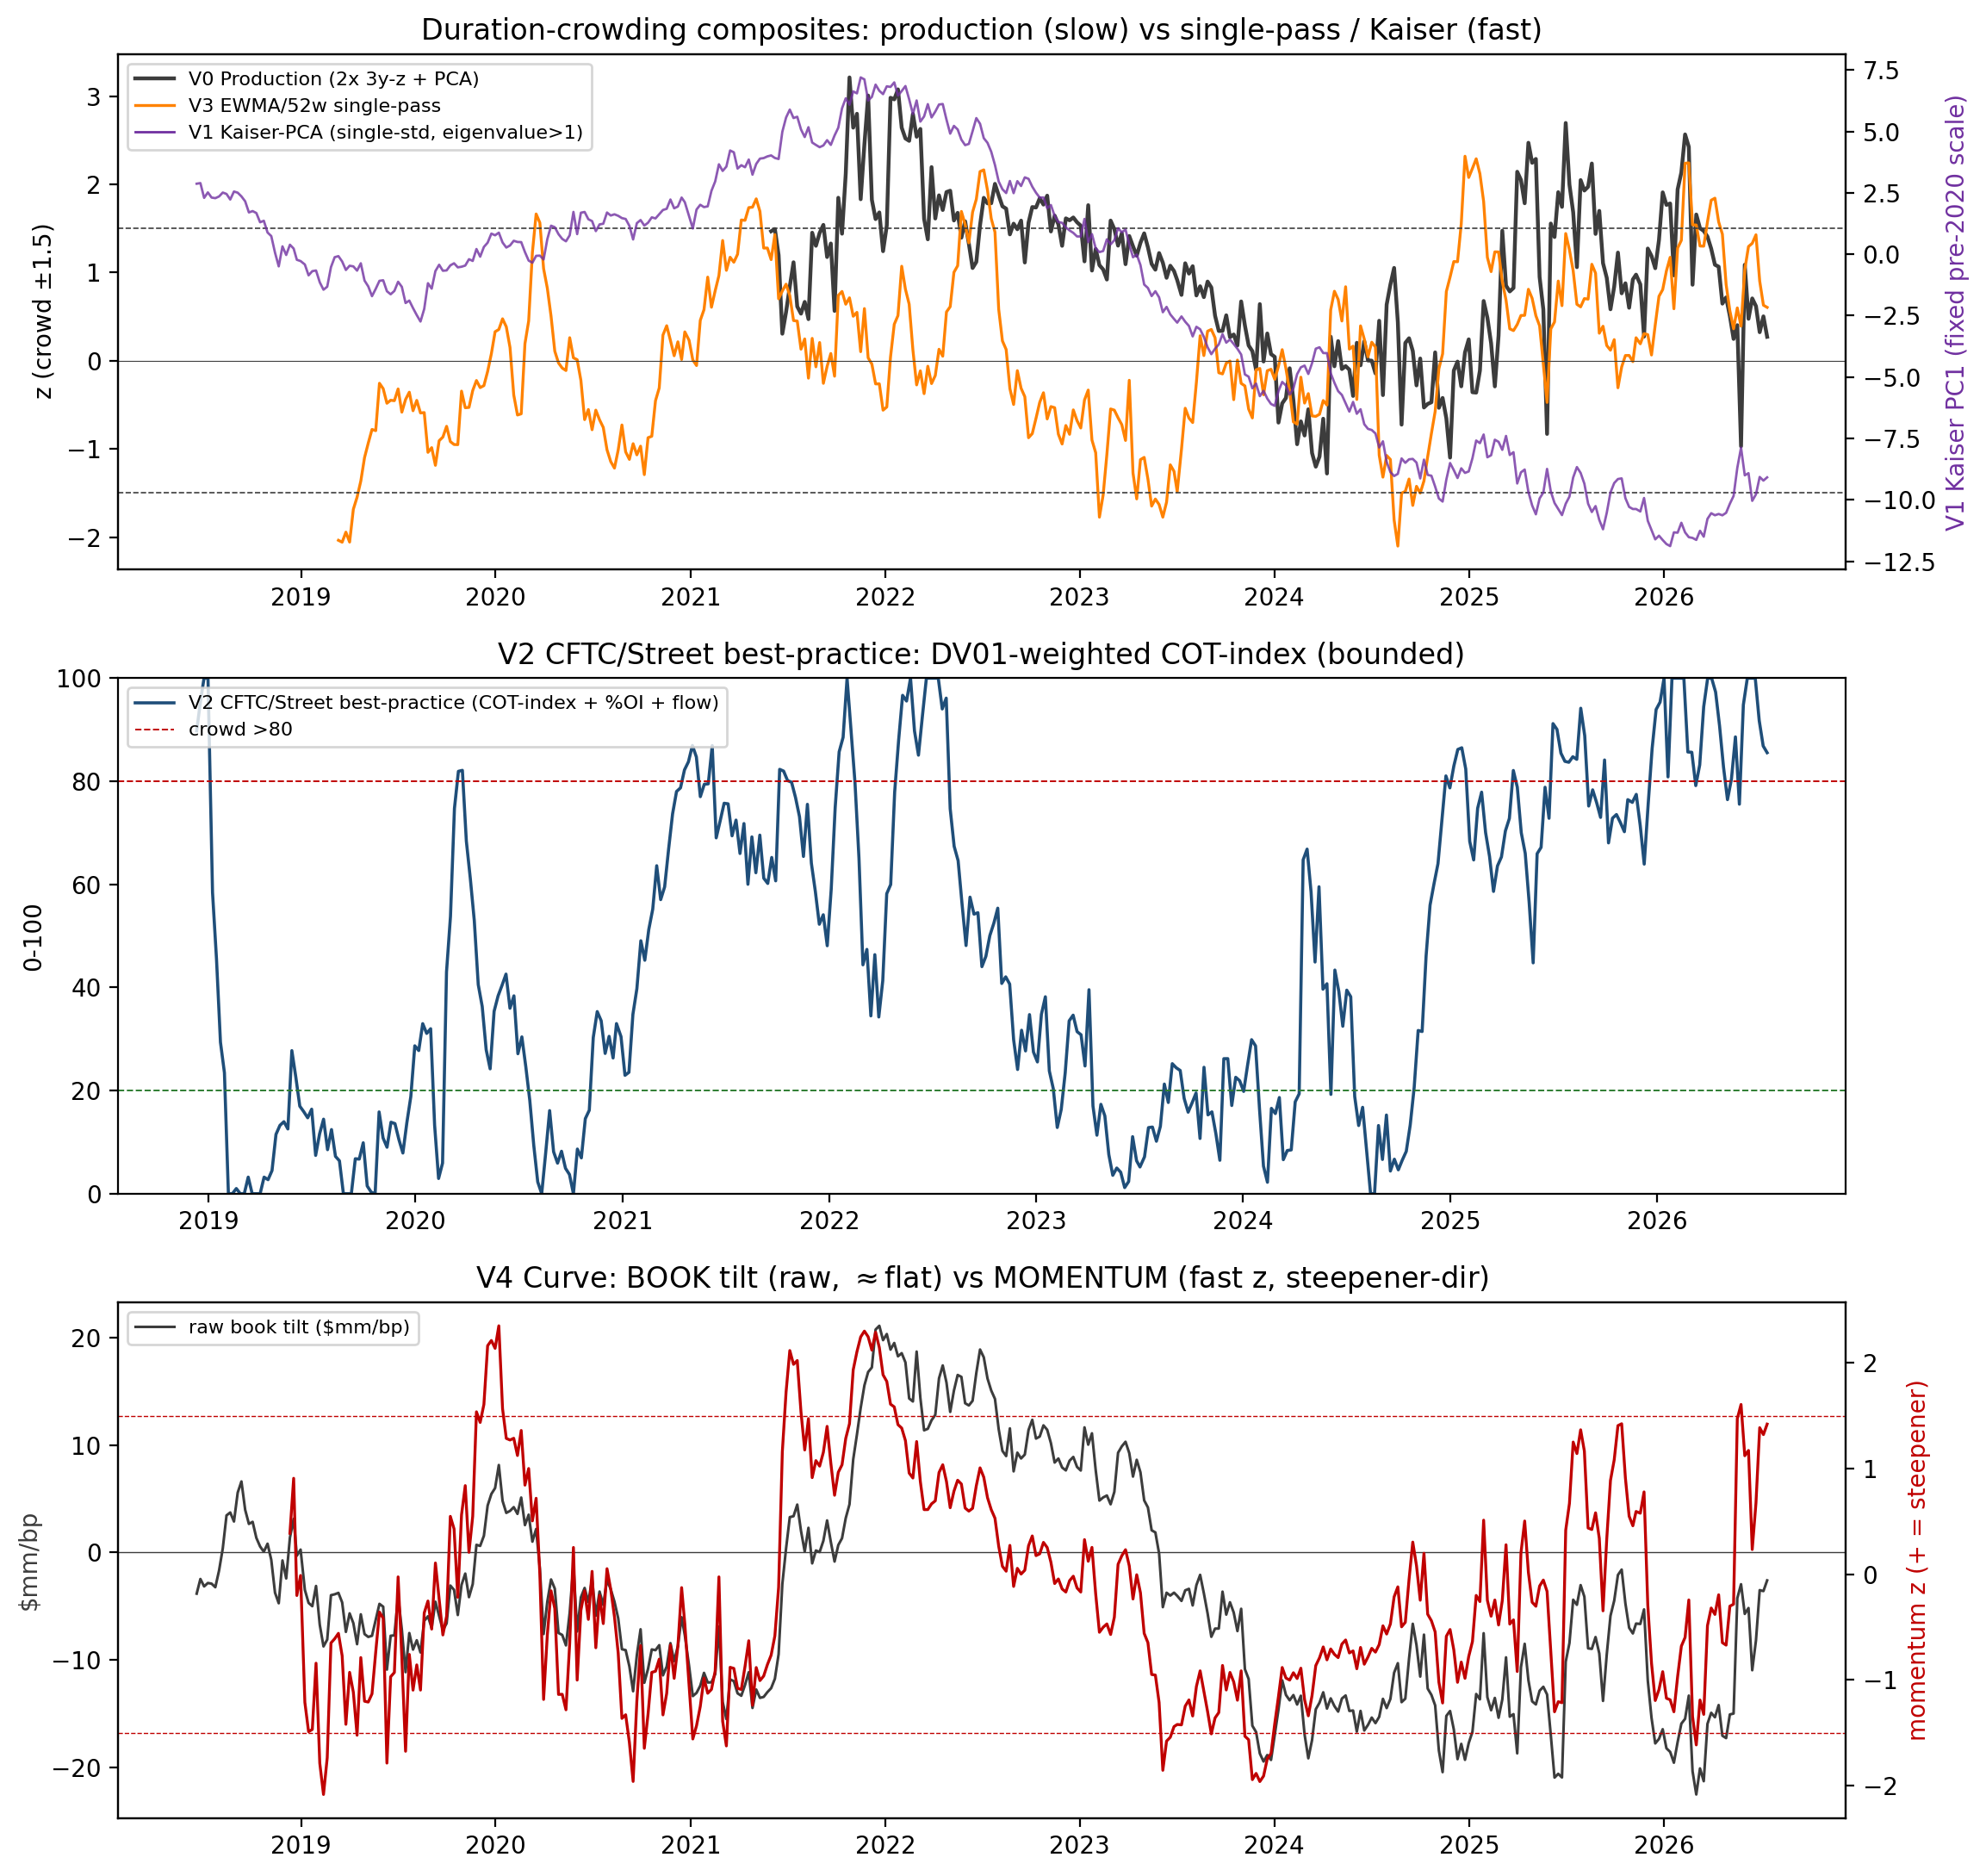
\includegraphics[width=0.96\textwidth]{fig_versions_overlay.png}
\caption*{\footnotesize\textbf{Fig 1.} Top: duration-crowding composites --- production (grey, slow) vs
EWMA/52w (orange) with Kaiser-PC1 on the right axis (fixed pre-2020 scale, hence the upward drift).
Middle: V2 bounded COT-index (saturates fast, crowd $>$80). Bottom: V4 curve --- raw book tilt
($\approx$flat now) vs momentum (steepener-direction).}\end{figure}

\sect{4. Recommendation}
Keep the tool's DV01 weighting and PCA (already OFR / Litterman-Scheinkman best practice); change only the
normalization, and offer the versions as selectable:
\begin{itemize}[leftmargin=1.4em]
\item \textbf{Headline, magnitude-comparable, fast:} \textbf{V3} (single-pass EWMA/52w) --- same $\pm$z
scale as today, $\sim$17 months faster, trivially simple.
\item \textbf{Desk-friendly bounded gauge:} \textbf{V2} COT-index (0--100, crowd $>$80) as a secondary
read --- matches how the Street quotes crowding; accept that it saturates.
\item \textbf{Factor view:} \textbf{V1} Kaiser-PCA for the ``distance from pre-2020 normal'' --- most
principled on the double-z fix, but present its magnitude with the fixed-scale caveat.
\item \textbf{Structural context:} keep \textbf{V0} 3y as a slow band, not the headline.
\item \textbf{Curve:} adopt \textbf{V4}'s two-series read (book tilt + momentum) everywhere the single
$z$ misled.
\end{itemize}
\textbf{Honesty note.} These are \emph{normalization} choices --- they change \emph{when} a given book is
called crowded, not whether crowding predicts returns (which the earlier study showed is weak: CIs
include 0.5). A faster flag is a better \emph{descriptor}, not new alpha. Production default remains V0
until a switch is chosen; \code{get\_composite("v1".."v4")} exposes each.

\vspace{4pt}{\footnotesize\color{biggrey}Reproduce: \code{python -m positioning.versions.compare}
(figures $+$ \code{versions\_compare.json}); each version self-runs via
\code{python -m positioning.versions.vX}. Built concurrently by four agents against
\code{positioning/versions/base.py}; \code{positioning/core} and \code{positioning\_score.json}
unchanged. Methodology sources in the companion note \code{positioning\_methodology\_review.pdf}.}
\end{document}
